\documentclass[conference,onecolumn]{IEEEtran}
\usepackage[T1]{fontenc}
\usepackage{longtable,booktabs,array,amsmath,graphicx}
\usepackage[hidelinks]{hyperref}
\newcommand{\checkpointrows}{%
B0 best & 12 & 81.06 & 77.12 \\
B0 last available & 14 & 80.77 & 76.08 \\
R1 best & 27 & 79.53 & 71.93 \\
R2 best & 28 & 80.49 & 72.76 \\
R1 final & 100 & 74.00 & 64.29 \\
R2 final & 100 & 71.37 & 62.72 \\%
}
\newcommand{\posttrainingrows}{%
Cosine & 74.00 & 70.80 & 64.29 & 62.84 & 71.37 & 68.15 & 62.72 & 61.59 \\
AQE & 76.41 & 73.81 & 65.90 & 64.84 & 73.64 & 70.86 & 64.06 & 63.36 \\
$\alpha$-QE & 76.45 & 73.86 & 65.89 & 64.83 & 73.63 & 70.90 & 64.06 & 63.36 \\
Gated QE & 76.45 & 73.86 & 65.89 & 64.83 & 73.63 & 70.90 & 64.06 & 63.36 \\
Local re-rank & 78.53 & 75.08 & 65.42 & 64.01 & 76.55 & 73.35 & 63.92 & 62.83 \\
Geometric re-rank & 76.68 & 73.46 & 64.83 & 63.40 & 74.98 & 71.84 & 63.33 & 62.19 \\
Verified QE & 78.94 & 76.28 & 66.97 & 65.82 & 76.85 & 74.25 & 65.10 & 64.31 \\
Mutual diffusion & 48.95 & 47.32 & 53.11 & 52.26 & 51.15 & 49.63 & 52.55 & 52.01 \\
Union diffusion & 23.67 & 22.10 & 45.61 & 45.15 & 25.79 & 24.13 & 46.15 & 46.05 \\%
}
\newcommand{\fusionrows}{%
Score fusion & 73.55 & 70.40 & 64.04 & 62.77 \\
RRF & 73.43 & 70.25 & 64.11 & 62.80 \\%
}
\newcommand{\sensitivityrows}{%
R1+R2 & Ox & RRF & c=100 & 73.41 \\
R1+R2 & Ox & RRF & c=10 & 73.56 \\
R1+R2 & Pa & RRF & c=100 & 64.08 \\
R1+R2 & Pa & RRF & c=10 & 64.13 \\
R1 & Ox & $\alpha$-QE & k=10, alpha=3, lam=0.25 & 75.58 \\
R1 & Ox & $\alpha$-QE & k=10, alpha=3, lam=1 & 77.30 \\
R1 & Ox & $\alpha$-QE & k=10, alpha=5, lam=0.5 & 76.54 \\
R1 & Ox & $\alpha$-QE & k=10, alpha=1, lam=0.5 & 76.42 \\
R1 & Ox & $\alpha$-QE & k=20, alpha=3, lam=0.5 & 75.52 \\
R1 & Ox & $\alpha$-QE & k=5, alpha=3, lam=0.5 & 77.15 \\
R1 & Ox & Mutual diffusion & k=40, beta=0.9 & 48.66 \\
R1 & Ox & Mutual diffusion & k=10, beta=0.9 & 55.91 \\
R1 & Ox & Mutual diffusion & k=20, beta=0.5 & 68.46 \\
R1 & Ox & Mutual diffusion & k=20, beta=0.99 & 28.16 \\
R1 & Ox & Union diffusion & k=40, beta=0.9 & 18.16 \\
R1 & Ox & Union diffusion & k=10, beta=0.9 & 29.12 \\
R1 & Ox & Union diffusion & k=20, beta=0.5 & 58.00 \\
R1 & Ox & Union diffusion & k=20, beta=0.99 & 8.43 \\
R1 & Ox & Gated QE & k=10, alpha=3, lam=0.5, tau=0.4 & 76.45 \\
R1 & Ox & Gated QE & k=10, alpha=3, lam=0.5, tau=0.6 & 76.45 \\
R1 & Ox & Geometric re-rank & k=50, eta=0.25 & 76.74 \\
R1 & Ox & Geometric re-rank & k=20, eta=0.5 & 74.86 \\
R1 & Ox & Geometric re-rank & k=50, eta=0.75 & 76.64 \\
R1 & Ox & Geometric re-rank & k=100, eta=0.5 & 77.37 \\
R1 & Ox & Local re-rank & k=50, eta=0.25 & 78.95 \\
R1 & Ox & Local re-rank & k=20, eta=0.5 & 75.99 \\
R1 & Ox & Local re-rank & k=50, eta=0.75 & 78.23 \\
R1 & Ox & Local re-rank & k=100, eta=0.5 & 78.85 \\
R1 & Pa & $\alpha$-QE & k=10, alpha=3, lam=0.25 & 65.27 \\
R1 & Pa & $\alpha$-QE & k=10, alpha=3, lam=1 & 66.56 \\
R1 & Pa & $\alpha$-QE & k=10, alpha=5, lam=0.5 & 65.89 \\
R1 & Pa & $\alpha$-QE & k=10, alpha=1, lam=0.5 & 65.90 \\
R1 & Pa & $\alpha$-QE & k=20, alpha=3, lam=0.5 & 65.86 \\
R1 & Pa & $\alpha$-QE & k=5, alpha=3, lam=0.5 & 65.71 \\
R1 & Pa & Mutual diffusion & k=40, beta=0.9 & 54.74 \\
R1 & Pa & Mutual diffusion & k=10, beta=0.9 & 49.36 \\
R1 & Pa & Mutual diffusion & k=20, beta=0.5 & 60.68 \\
R1 & Pa & Mutual diffusion & k=20, beta=0.99 & 41.93 \\
R1 & Pa & Union diffusion & k=40, beta=0.9 & 41.45 \\
R1 & Pa & Union diffusion & k=10, beta=0.9 & 46.28 \\
R1 & Pa & Union diffusion & k=20, beta=0.5 & 58.57 \\
R1 & Pa & Union diffusion & k=20, beta=0.99 & 20.59 \\
R1 & Pa & Gated QE & k=10, alpha=3, lam=0.5, tau=0.4 & 65.89 \\
R1 & Pa & Gated QE & k=10, alpha=3, lam=0.5, tau=0.6 & 65.89 \\
R1 & Pa & Geometric re-rank & k=50, eta=0.25 & 64.83 \\
R1 & Pa & Geometric re-rank & k=20, eta=0.5 & 64.44 \\
R1 & Pa & Geometric re-rank & k=50, eta=0.75 & 64.83 \\
R1 & Pa & Geometric re-rank & k=100, eta=0.5 & 65.55 \\
R1 & Pa & Local re-rank & k=50, eta=0.25 & 65.42 \\
R1 & Pa & Local re-rank & k=20, eta=0.5 & 64.55 \\
R1 & Pa & Local re-rank & k=50, eta=0.75 & 65.42 \\
R1 & Pa & Local re-rank & k=100, eta=0.5 & 66.94 \\
R2 & Ox & $\alpha$-QE & k=10, alpha=3, lam=0.25 & 72.96 \\
R2 & Ox & $\alpha$-QE & k=10, alpha=3, lam=1 & 74.32 \\
R2 & Ox & $\alpha$-QE & k=10, alpha=5, lam=0.5 & 73.64 \\
R2 & Ox & $\alpha$-QE & k=10, alpha=1, lam=0.5 & 73.63 \\
R2 & Ox & $\alpha$-QE & k=20, alpha=3, lam=0.5 & 72.48 \\
R2 & Ox & $\alpha$-QE & k=5, alpha=3, lam=0.5 & 74.01 \\
R2 & Ox & Mutual diffusion & k=40, beta=0.9 & 50.41 \\
R2 & Ox & Mutual diffusion & k=10, beta=0.9 & 56.04 \\
R2 & Ox & Mutual diffusion & k=20, beta=0.5 & 66.58 \\
R2 & Ox & Mutual diffusion & k=20, beta=0.99 & 29.29 \\
R2 & Ox & Union diffusion & k=40, beta=0.9 & 20.24 \\
R2 & Ox & Union diffusion & k=10, beta=0.9 & 30.51 \\
R2 & Ox & Union diffusion & k=20, beta=0.5 & 57.81 \\
R2 & Ox & Union diffusion & k=20, beta=0.99 & 9.14 \\
R2 & Ox & Gated QE & k=10, alpha=3, lam=0.5, tau=0.4 & 73.63 \\
R2 & Ox & Gated QE & k=10, alpha=3, lam=0.5, tau=0.6 & 73.63 \\
R2 & Ox & Geometric re-rank & k=50, eta=0.25 & 75.04 \\
R2 & Ox & Geometric re-rank & k=20, eta=0.5 & 73.48 \\
R2 & Ox & Geometric re-rank & k=50, eta=0.75 & 74.94 \\
R2 & Ox & Geometric re-rank & k=100, eta=0.5 & 75.68 \\
R2 & Ox & Local re-rank & k=50, eta=0.25 & 76.90 \\
R2 & Ox & Local re-rank & k=20, eta=0.5 & 74.18 \\
R2 & Ox & Local re-rank & k=50, eta=0.75 & 76.36 \\
R2 & Ox & Local re-rank & k=100, eta=0.5 & 77.29 \\
R2 & Pa & $\alpha$-QE & k=10, alpha=3, lam=0.25 & 63.55 \\
R2 & Pa & $\alpha$-QE & k=10, alpha=3, lam=1 & 64.63 \\
R2 & Pa & $\alpha$-QE & k=10, alpha=5, lam=0.5 & 64.06 \\
R2 & Pa & $\alpha$-QE & k=10, alpha=1, lam=0.5 & 64.07 \\
R2 & Pa & $\alpha$-QE & k=20, alpha=3, lam=0.5 & 64.33 \\
R2 & Pa & $\alpha$-QE & k=5, alpha=3, lam=0.5 & 64.10 \\
R2 & Pa & Mutual diffusion & k=40, beta=0.9 & 53.81 \\
R2 & Pa & Mutual diffusion & k=10, beta=0.9 & 50.17 \\
R2 & Pa & Mutual diffusion & k=20, beta=0.5 & 59.46 \\
R2 & Pa & Mutual diffusion & k=20, beta=0.99 & 41.94 \\
R2 & Pa & Union diffusion & k=40, beta=0.9 & 41.77 \\
R2 & Pa & Union diffusion & k=10, beta=0.9 & 46.51 \\
R2 & Pa & Union diffusion & k=20, beta=0.5 & 58.14 \\
R2 & Pa & Union diffusion & k=20, beta=0.99 & 20.03 \\
R2 & Pa & Gated QE & k=10, alpha=3, lam=0.5, tau=0.4 & 64.06 \\
R2 & Pa & Gated QE & k=10, alpha=3, lam=0.5, tau=0.6 & 64.06 \\
R2 & Pa & Geometric re-rank & k=50, eta=0.25 & 63.33 \\
R2 & Pa & Geometric re-rank & k=20, eta=0.5 & 62.85 \\
R2 & Pa & Geometric re-rank & k=50, eta=0.75 & 63.33 \\
R2 & Pa & Geometric re-rank & k=100, eta=0.5 & 64.24 \\
R2 & Pa & Local re-rank & k=50, eta=0.25 & 63.93 \\
R2 & Pa & Local re-rank & k=20, eta=0.5 & 62.99 \\
R2 & Pa & Local re-rank & k=50, eta=0.75 & 63.92 \\
R2 & Pa & Local re-rank & k=100, eta=0.5 & 65.55 \\%
}
\newcommand{\secondaryrows}{%
R1+R2 & Ox & RRF & 79.66 & 48.98 & 67.05 & 77.00 & 50.83 \\
R1+R2 & Ox & score\_fusion & 79.92 & 48.92 & 67.05 & 77.07 & 50.93 \\
R1+R2 & Pa & RRF & 91.68 & 13.93 & 30.05 & 48.78 & 55.16 \\
R1+R2 & Pa & score\_fusion & 91.72 & 13.94 & 30.07 & 48.80 & 55.25 \\
R1 & Ox & AQE & 81.05 & 50.96 & 68.79 & 78.68 & 55.28 \\
R1 & Ox & $\alpha$-QE & 81.11 & 50.98 & 68.80 & 78.67 & 55.32 \\
R1 & Ox & Cosine & 79.21 & 48.98 & 66.88 & 77.30 & 48.33 \\
R1 & Ox & Mutual diffusion & 67.70 & 34.32 & 47.92 & 58.71 & 37.96 \\
R1 & Ox & Union diffusion & 29.77 & 8.89 & 20.35 & 32.58 & 13.46 \\
R1 & Ox & Gated QE & 81.11 & 50.98 & 68.80 & 78.67 & 55.32 \\
R1 & Ox & Geometric re-rank & 82.65 & 50.67 & 66.88 & 77.30 & 54.17 \\
R1 & Ox & Local re-rank & 84.22 & 52.34 & 66.88 & 77.30 & 55.96 \\
R1 & Ox & Verified QE & 83.58 & 52.70 & 69.83 & 79.41 & 60.97 \\
R1 & Pa & AQE & 92.26 & 14.13 & 30.33 & 50.13 & 58.17 \\
R1 & Pa & $\alpha$-QE & 92.27 & 14.13 & 30.33 & 50.12 & 58.17 \\
R1 & Pa & Cosine & 91.18 & 13.90 & 29.59 & 48.74 & 54.71 \\
R1 & Pa & Mutual diffusion & 88.32 & 13.36 & 27.88 & 42.15 & 46.49 \\
R1 & Pa & Union diffusion & 69.08 & 9.87 & 21.04 & 35.19 & 40.68 \\
R1 & Pa & Gated QE & 92.27 & 14.13 & 30.33 & 50.12 & 58.17 \\
R1 & Pa & Geometric re-rank & 94.40 & 14.28 & 29.59 & 48.74 & 55.13 \\
R1 & Pa & Local re-rank & 96.41 & 14.90 & 29.59 & 48.74 & 55.67 \\
R1 & Pa & Verified QE & 94.17 & 14.37 & 30.73 & 50.70 & 58.60 \\
R2 & Ox & AQE & 79.81 & 49.28 & 66.89 & 77.32 & 57.29 \\
R2 & Ox & $\alpha$-QE & 79.86 & 49.31 & 66.93 & 77.33 & 57.35 \\
R2 & Ox & Cosine & 78.66 & 48.07 & 65.45 & 75.69 & 50.91 \\
R2 & Ox & Mutual diffusion & 69.15 & 35.77 & 51.19 & 59.94 & 42.50 \\
R2 & Ox & Union diffusion & 30.02 & 10.28 & 22.74 & 38.98 & 15.59 \\
R2 & Ox & Gated QE & 79.86 & 49.31 & 66.93 & 77.33 & 57.35 \\
R2 & Ox & Geometric re-rank & 82.70 & 49.73 & 65.45 & 75.69 & 56.83 \\
R2 & Ox & Local re-rank & 83.85 & 51.32 & 65.45 & 75.69 & 57.68 \\
R2 & Ox & Verified QE & 82.87 & 51.49 & 68.88 & 78.35 & 60.88 \\
R2 & Pa & AQE & 92.49 & 14.08 & 30.58 & 49.48 & 57.70 \\
R2 & Pa & $\alpha$-QE & 92.52 & 14.08 & 30.57 & 49.48 & 57.70 \\
R2 & Pa & Cosine & 91.71 & 13.89 & 29.87 & 48.28 & 54.40 \\
R2 & Pa & Mutual diffusion & 88.25 & 13.15 & 27.72 & 41.88 & 47.38 \\
R2 & Pa & Union diffusion & 70.19 & 10.21 & 22.05 & 36.69 & 42.74 \\
R2 & Pa & Gated QE & 92.52 & 14.08 & 30.57 & 49.48 & 57.70 \\
R2 & Pa & Geometric re-rank & 94.71 & 14.32 & 29.87 & 48.28 & 54.77 \\
R2 & Pa & Local re-rank & 96.31 & 15.05 & 29.87 & 48.28 & 55.11 \\
R2 & Pa & Verified QE & 94.40 & 14.30 & 30.99 & 50.04 & 57.75 \\%
}

\setcounter{LTchunksize}{200}
\begin{document}
\title{Supplementary Results: Training and Post-Training Strategies for VGG16--GeM Image Retrieval}
\author{\IEEEauthorblockN{Author 1 \qquad Author 2 \qquad Author 3}}
\maketitle
\section{Scope and Reading Guide}
This supplement preserves all 100 additional clean sensitivity configurations and secondary metrics for all 40 main model--dataset--method groups. R1 denotes augmentation-only, R2 augmentation plus the spatial gate, and R1+R2 their fusion. Both search encoders are fixed at epoch 100 with FP32 extraction. Ox and Pa denote legacy Oxford5k and Paris6k. All score entries are percentages. The main paper reports the frozen reference settings; these additional sensitivity results are exploratory test observations and were not used to replace the corruption settings.

\section{Illustrative Retrieval Cases}
Figure~\ref{fig:cases} displays the largest and smallest AP changes from verified QE among the 55 R1 Oxford queries under the fixed blur-severity-three condition. This is an explicit extreme-case selection, not a representative random sample. The largest gain is for \texttt{pitt\_rivers\_000087}: AP increases from 0.4545 to 0.9742. The minimum change is zero; the illustrated \texttt{all\_souls\_000013} case remains at AP 0.4200. Thus the second row illustrates a difficult query that is not recovered, rather than a negative AP change. The source query may appear in the gallery under the legacy protocol.
\begin{figure}[ht]
\centering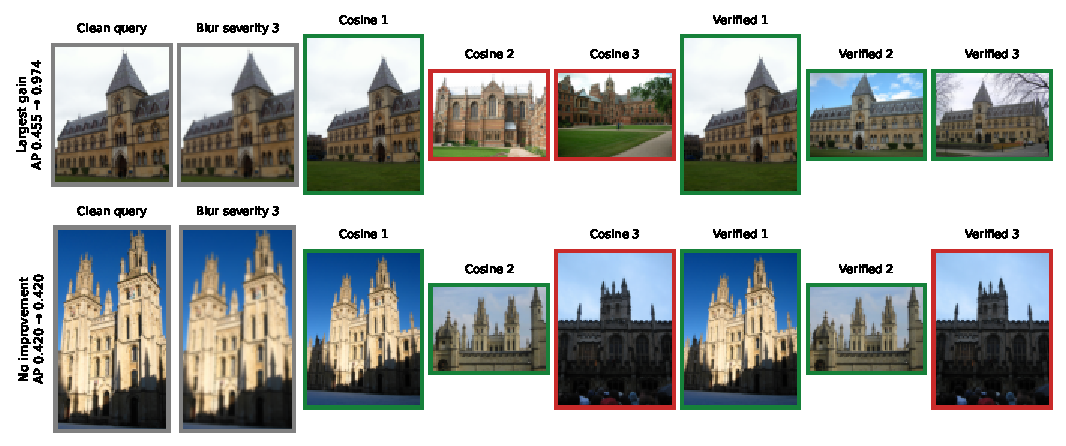
\includegraphics[width=0.98\textwidth]{figures/qualitative_cases.pdf}
\caption{Clean query, corrupted query, and the first three non-junk results from cosine and verified QE. Green borders mark relevant gallery images and red borders non-relevant images, using ground truth only for this post-hoc visualization. Labels and the complete query/image IDs are saved in \texttt{data/qualitative\_cases.json}.}
\label{fig:cases}
\end{figure}

\clearpage
\section{Complete Clean Sensitivity}
Each row averages AP over 55 queries. The 100 rows correspond to 5,500 query AP values. Only the displayed axes vary from the method's frozen reference; other parameters remain fixed. QE uses a residual query with normalized feedback. Here \texttt{lam} is lambda, \texttt{tau} the cosine gate, and \texttt{k} the feedback, candidate, or graph-neighbor count according to the method.
{\small
\begin{longtable}{p{0.07\textwidth}p{0.04\textwidth}p{0.19\textwidth}p{0.45\textwidth}r}
\caption{All additional clean sensitivity results.}\\
\toprule Model & Set & Method & Parameters & mAP \\
\midrule\endfirsthead
\toprule Model & Set & Method & Parameters & mAP \\
\midrule\endhead
\bottomrule\endfoot
\sensitivityrows
\end{longtable}}

\clearpage
\section{Secondary Main-Protocol Metrics}
P@10 and relevant Recall@20/50/100 remove junk before truncating rankings. Recall is the fraction of all relevant gallery images recovered, not a binary success indicator. To preserve the saved summary convention, precision and recall average clean plus the 18 corrupted family--severity conditions equally, after realization averaging. Worst is the minimum among the 18 corrupted condition-level mAP values; it excludes clean.
{\small
\begin{longtable}{lllrrrrr}
\caption{Clean-plus-corrupted precision/recall and corrupted worst-condition mAP.}\\
\toprule Model & Set & Method & P@10 & R@20 & R@50 & R@100 & Worst \\
\midrule\endfirsthead
\toprule Model & Set & Method & P@10 & R@20 & R@50 & R@100 & Worst \\
\midrule\endhead
\bottomrule\endfoot
\secondaryrows
\end{longtable}}
\section{Machine-Readable Evidence}
The accompanying source package contains the complete clean checkpoint comparison, 40 main summary rows, 100 sensitivity rows with full JSON configurations, the 214-epoch combined history, condition-level scores, direct end-to-end latency medians and p95, and diagnostics. The evidence manifest records source hashes. Retrieval-only timings in the summary and direct end-to-end timings in the latency table are different quantities and should not be combined as if they were additive components.
\end{document}
